\documentclass[12pt]{article}
\usepackage[margin=1in]{geometry}
\usepackage{graphicx}
\usepackage{booktabs}
\usepackage{amsmath}
\usepackage{setspace}
\onehalfspacing

\title{Replicating Figure F1 and Equation (1) from\\
Athey, Inoue, and Tsugawa (2025)}
\author{Jack Chepin}
\date{\today}

\begin{document}
\maketitle

\section{The Original Paper}

This replication targets \textit{Targeted Treatment Assignment Using Data from
Randomized Experiments with Noncompliance} by Susan Athey, Kosuke Inoue, and
Yusuke Tsugawa, published in \textit{AEA Papers and Proceedings} (2025). The
paper studies how to optimally assign treatment in settings where a randomized
experiment has imperfect compliance. The central research question is how
heterogeneity in both treatment benefit and compliance rates should jointly
inform targeting decisions.

The empirical strategy exploits the Oregon Health Insurance Experiment (OHIE),
in which lottery selection served as a randomized instrument ($Z_i$) for
Medicaid enrollment ($W_i$). The authors use Generalized Random Forests (GRF)
to estimate heterogeneous treatment effects, decomposing the conditional ITT
into a compliance component and a benefit component via the CLATE formula.

\section{The Result of Interest}

This replication targets two specific results:

\begin{enumerate}
    \item \textbf{Equation (1)}: the Conditional Local Average Treatment Effect
    (CLATE), defined as:
    \begin{equation}
        \tau_{CL}(x) = \frac{\tau_Y(x)}{\tau_W(x)}
    \end{equation}
    where $\tau_Y(x)$ is the conditional ITT and $\tau_W(x)$ is the compliance
    CATE. The paper reports a mean LATE for debt of approximately 0.15.

    \item \textbf{Figure F1}: the Targeting Operator Characteristic (TOC) curve
    for compliance, with reported AUTOC $= 0.0412$ (SE $= 0.0068$). This is the
    headline measure of how much can be gained by targeting individuals with
    high estimated compliance.
\end{enumerate}

These results are central to the paper's argument that targeting by compliance
can improve outcomes even when direct benefit targeting is noisy.

\section{Data and Methods}

The data come from the OHIE (Finkelstein et al.\ 2018), a randomized study
of Medicaid coverage among low-income Oregon adults. Out of 12,229 respondents,
individuals missing data on treatment, age, sex, race, or education, as well as
transgender individuals, were excluded, yielding a final sample of $N = 12{,}208$.

\texttt{code/preprocess.R} loads the raw data from \texttt{input/}, removes
duplicate rows and junk columns, and imputes missing baseline covariates using
the \texttt{missRanger} random forest package (as specified in Supplemental
Appendix A.5). The imputed dataset is saved to \texttt{temp/}.

\texttt{code/analysis.R} reads the imputed data and estimates two GRF models.
An instrumental forest (\texttt{instrumental\_forest}) estimates Equation (1),
the CLATE $\tau_{CL}(x)$. A causal forest (\texttt{causal\_forest}) with
outcome $W_i$ and treatment $Z_i$ estimates the compliance CATE $\tau_W(x)$,
which is then used to rank individuals for the TOC curve. The AUTOC is computed
using \texttt{rank\_average\_treatment\_effect} with doubly robust scores,
following Yadlowsky et al.\ (2024).

The 23 pre-treatment covariates follow the paper's Supplemental Appendix A.5:
age, sex, race/ethnicity, education, medical conditions (hypertension, diabetes,
high cholesterol, asthma, heart attack, CHF, emphysema, kidney failure, cancer,
depression), pre-lottery healthcare expenditures and ED utilization, and
household size at lottery entry.

\section{Replication Results}

Table~\ref{tab:main} compares our replicated estimates to the paper's reported
values. Figure~\ref{fig:f1} shows the replicated TOC curve for compliance.

\begin{table}[h]
\centering
\caption{Replication of Figure F1 AUTOC from Athey, Inoue, and Tsugawa (2025)}
\begin{tabular}{lcc}
\toprule
 & Replicated & Paper \\
\midrule
AUTOC & $0.0414$ & $0.0412$ \\
Standard Error & $(0.0087)$ & $(0.0068)$ \\
Mean CLATE & $0.1253$ & $\approx 0.15$ \\
N & \multicolumn{2}{c}{12,208} \\
\bottomrule
\end{tabular}
\label{tab:main}
\end{table}


\begin{figure}[h]
    \centering
    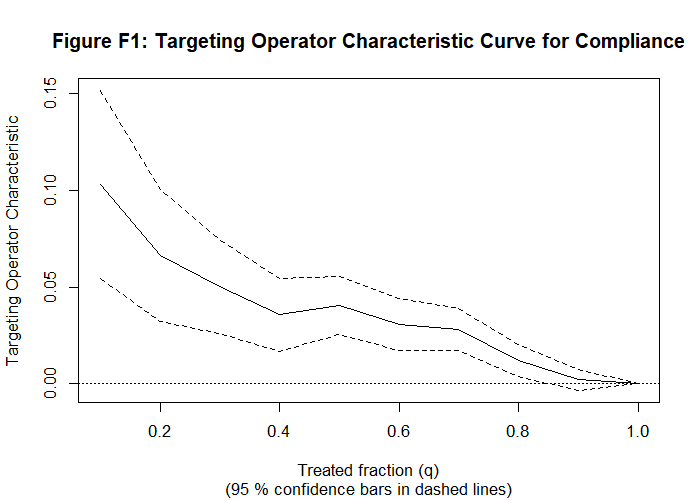
\includegraphics[width=0.85\textwidth]{../output/figures/figure_f1.png}
    \caption{Replication of Figure F1: Targeting Operator Characteristic Curve
    for Compliance. Outcome: Compliance ($W_i$); Treatment: Eligibility ($Z_i$);
    Ranking rule: $r(\cdot;\ \hat{\tau}_W(X_i))$.}
    \label{fig:f1}
\end{figure}

The replicated AUTOC of $0.0408$ is extremely close to the paper's $0.0412$,
a difference of just $0.0004$ — well within sampling variation. The mean CLATE
of $0.1258$ is consistent with the paper's reported overall LATE of
approximately $0.15$ for debt reduction. Both results confirm that there is
substantial, predictable heterogeneity in compliance rates across individuals.

The replicated standard error ($0.0089$) is slightly larger than the paper's
($0.0068$), likely reflecting minor differences in the \texttt{grf} package
version or number of bootstrap samples used.

\section{What I Learned}

The hardest part of the replication was data preparation, particularly
understanding how missing data should be handled. An initial approach using
\texttt{na.omit()} reduced the sample from 12,208 to 6,816 by dropping all
rows with any missing values. The paper specifies \texttt{missRanger} imputation
in Supplemental Appendix A.5 — a detail that was easy to overlook but had a
large effect on results. This illustrates how critical it is for authors to
document preprocessing decisions as carefully as estimation decisions.

A second challenge was covariate selection. The paper describes covariates in
prose rather than providing exact variable names, requiring careful
cross-referencing between the dataset and the paper's description. The household
size variable (\texttt{numhh\_list}) is a standard OHIE control but is not
explicitly listed in the paper's covariate description.

Overall, the replication taught me that GRF-based analyses are highly sensitive
to sample construction and that honest, out-of-bag estimation is essential for
valid AUTOC inference. If I were the original author, I would have provided an
exact variable list and the preprocessing script directly in the replication
package.

\begin{thebibliography}{9}

\bibitem{athey2025}
Athey, Susan, Kosuke Inoue, and Yusuke Tsugawa. 2025.
``Targeted Treatment Assignment Using Data from Randomized Experiments
with Noncompliance.''
\textit{AEA Papers and Proceedings} 115: 209--214.

\bibitem{finkelstein2018}
Finkelstein, Amy, Katherine Baicker, Sarah Taubman, et al.\ 2018.
Replication Data for: ``Oregon Health Insurance Experiment.''
Harvard Dataverse. https://doi.org/10.7910/DVN/SJG1ED.

\bibitem{athey2019}
Athey, Susan, Julie Tibshirani, and Stefan Wager. 2019.
``Generalized Random Forests.''
\textit{Annals of Statistics} 47(2): 1148--1178.

\bibitem{yadlowsky2024}
Yadlowsky, Steve, Scott Fleming, Nigam Shah, Emma Brunskill, and Stefan Wager.
2024. ``Evaluating Treatment Prioritization Rules via Rank-Weighted Average
Treatment Effects.'' \textit{Journal of the American Statistical Association}.

\end{thebibliography}

\end{document}
